
%% bare_conf_compsoc.tex
%% V1.4b
%% 2015/08/26
%% by Michael Shell
%% See:
%% http://www.michaelshell.org/
%% for current contact information.
%%
%% This is a skeleton file demonstrating the use of IEEEtran.cls
%% (requires IEEEtran.cls version 1.8b or later) with an IEEE Computer
%% Society conference paper.
%%
%% Support sites:
%% http://www.michaelshell.org/tex/ieeetran/
%% http://www.ctan.org/pkg/ieeetran
%% and
%% http://www.ieee.org/

%%*************************************************************************
%% Legal Notice:
%% This code is offered as-is without any warranty either expressed or
%% implied; without even the implied warranty of MERCHANTABILITY or
%% FITNESS FOR A PARTICULAR PURPOSE! 
%% User assumes all risk.
%% In no event shall the IEEE or any contributor to this code be liable for
%% any damages or losses, including, but not limited to, incidental,
%% consequential, or any other damages, resulting from the use or misuse
%% of any information contained here.
%%
%% All comments are the opinions of their respective authors and are not
%% necessarily endorsed by the IEEE.
%%
%% This work is distributed under the LaTeX Project Public License (LPPL)
%% ( http://www.latex-project.org/ ) version 1.3, and may be freely used,
%% distributed and modified. A copy of the LPPL, version 1.3, is included
%% in the base LaTeX documentation of all distributions of LaTeX released
%% 2003/12/01 or later.
%% Retain all contribution notices and credits.
%% ** Modified files should be clearly indicated as such, including  **
%% ** renaming them and changing author support contact information. **
%%*************************************************************************


\documentclass[conference,compsoc,12pt]{IEEEtran}
%\documentclass[peerreview,12pt]{IEEEtran}

% *** CITATION PACKAGES ***
\usepackage[nocompress]{cite}

% *** GRAPHICS RELATED PACKAGES ***
%
\usepackage[pdftex]{graphicx}
% declare the path(s) where your graphic files are
%\graphicspath{{../images/}}
% and their extensions so you won't have to specify these with
% every instance of \includegraphics
%\DeclareGraphicsExtensions{.jpeg,.png}

% *** MATH PACKAGES ***
\usepackage{amsmath}
% Note that the amsmath package sets \interdisplaylinepenalty to 10000
% thus preventing page breaks from occurring within multiline equations. Use:
%\interdisplaylinepenalty=2500

% *** ALIGNMENT PACKAGES ***
\usepackage{array}

% *** SUBFIGURE PACKAGES ***
\usepackage[caption=false,font=footnotesize,labelfont=sf,textfont=sf]{subfig}

% *** FLOAT PACKAGES ***
%\usepackage{fixltx2e}
%\usepackage{stfloats}
% \usepackage{dblfloatfix}

% *** PDF, URL AND HYPERLINK PACKAGES ***
\usepackage{url}
\usepackage{bm}
%\usepackage{algorithm}
%\usepackage{algorithmic}

% *** Temporary packages ***
\usepackage{lipsum}
\usepackage{pifont}
\usepackage{mdframed}
\usepackage{float}

% Set figures and tables within text for peer-review
\makeatletter
\@ifclasswith{IEEEtran}{peerreview}{\floatplacement{figure}{H}}{\floatplacement{table}{H}}	
\makeatother

%\usepackage{xcolor}
%\newcommand\mytodo[1]{\textcolor{red}{#1}}

% correct bad hyphenation here
\hyphenation{op-tical net-works semi-conduc-tor}

\mdfsetup{%
	skipabove=0.5cm,
	innertopmargin=0.5cm,
	innerbottommargin=0.5cm
}

\begin{document}

% paper title
\title{Feature selection methods for machine learning based docking prediction of Indonesian medicinal plant compounds and HIV-1 protease}


% author names and affiliations
% use a multiple column layout for up to three different
% affiliations
%\author{
%	\IEEEauthorblockN{Rahman Pujianto}
%	\IEEEauthorblockA{Faculty of Computer Science\\
%	Universitas Indonesia\\
%	Email: rahman.pujianto@ui.ac.id\\}
%	\and
%	\IEEEauthorblockN{Heru Suhartanto}
%	\IEEEauthorblockA{Faculty of Computer Science\\
%	Universitas Indonesia\\
%	Email: heru@cs.ui.ac.id\\}
%}

\author{
	\IEEEauthorblockN{
		Rahman Pujianto\IEEEauthorrefmark{1},
		Yohanes Gultom\IEEEauthorrefmark{2}, 
		Ari Wibisono\IEEEauthorrefmark{3},		
		Heru Suhartanto\IEEEauthorrefmark{4}
	}
	\IEEEauthorblockA{
		Faculty of Computer Science,
		Universitas Indonesia\\
		Email: 
		\IEEEauthorrefmark{1}rahman.pujianto@ui.ac.id,
		\IEEEauthorrefmark{2}yohanes.gultom@ui.ac.id,
		\IEEEauthorrefmark{3}ari.w@cs.ui.ac.id 
		\IEEEauthorrefmark{4}heru@cs.ui.ac.id		
	}
}

% make the title area
\maketitle

% As a general rule, do not put math, special symbols or citations
% in the abstract
\begin{abstract}

This research evaluates usage feature selection methods to reduce number of features required to predict docking result between Indonesian medicinal plant compounds and HIV protease. Two feature selection methods, Recursive Feature Elimination (RFE) and Wrapper Method (WM), are trained with dataset of 7,331 samples and 667 features from PubChem Bioassay and DUD-E decoys. To evaluate the selected features, a dataset of 368 Indonesian herbal chemical compounds labeled by manually docking to PDB HIV-1 protease is used to benchmark the performance of linear SVM classifier using different sets of features. Our experiments show that set of 471 features selected by RFE and WM achieve reduction of classification time by 4.0 and 8.2 seconds respectively. Although the accuracy and sensitivity are also increased by 8\% and 16\%, no improvement observed for precision and specificity.  

\end{abstract}

\IEEEpeerreviewmaketitle

\section{Introduction}

The evolution of viruses can makes them resistant to existing drugs. One of the most popular case is HIV (Human Immunodeficiency Virus) which caused AIDS (Acquired Immunodeficiency Syndrome), which has been a global issue for years. HIV possesses a high drugs resistance due to its high replication and mutation abilities. Since drug discovery is a very complicated, expensive and time-consuming, curing AIDS and other illness caused by evolving virus become very challenging\cite{yanuar2014virtual}.

In order to discover new drugs, first, one needs to find a set of chemical compound candidates by observing reaction to drug target in the lab. This process is usually called high-throughput screening (HTS). Despite of its importance, this process is considered inefficient and expensive because most of chemical compounds consumed in the experiments. One way to make this process more efficient is by reducing the number of compounds that need to be tested in lab by performing virtual screening beforehand \cite{chen2017developing}. By having the number of lab experiments reduced, ultimately it will reduce overall time and cost needed in drug discovery \cite{korkmaz2014drug}.

Virtual screening applies computer algorithms to find chemical compounds that have high probability of reaction to drug's target. One of its approach is ligand-based screening (LBS), where new candidates are chosen based on their structural or characteristic similarity to known drug's chemical compounds. This implies that LBS approach relies on previous drug discovery results, which usually obtained using HTS such as PubChem BioAssay \cite{bioassay2014update}, CHEMBL \cite{bento2014chembl}, PubChem Compound \cite{kim2015pubchem} and ZINC \cite{irwin2012zinc}.

Since LBS is also a pattern matching problem, supervised learning algorithms can be used to classify chemical compounds using database of known drug descriptions as training dataset. The number of features required to described each compounds also affects the performance of both supervised and unsupervised learning algorithms. This phenomenon is usually addressed as the curse of dimensionality \cite{janecek2008relationship}. Two techniques commonly applied to solve this phenomenon are feature extraction and feature selection. While the first one extracts or processes existing features to get set of new ones, the last one selects a subset of features from the existing ones. This research focuses on observing the performance of two feature selection methods, SVM Recursive Feature Elimination (SVM-RFE) and Wrapper Method (WM), to select subset of features from Indonesian herbal chemical compounds that react to HIV-1 protease.

\section{Related Work}

Related research in virtual screening used a method that consist of two phases: First, machine learning based LBS is used to select potential chemical compound candidates, and second, molecular docking is done with between potential candidates and drug's target \cite{hilman2012analisis}. Since molecular docking requires a lot of computational resources, high LBS precision is required to improve efficiency. In the other hand, low recall or sensitivity causes potential candidates excluded \cite{korkmaz2014drug}. This research shows Support Vector Machine (SVM) performs well to classify potential candidates in LBS. Using this as basis, we explore usage of feature selections to improve SVM performance in LBS.

Molecular descriptor is a numerical value representing chemical information encoded within a symbolic representation of a molecule. This numerical value can also be obtained by some standardized experiment on a molecule \cite{yap2011padel}. At least there are 701 types of molecular descriptor that can be extracted from a chemical compounds. Therefore, it is difficult to analyze manually all correlations between descriptors \cite{korkmaz2014drug}. In machine learning based LBS, not all molecular descriptors directly affect the result of classification. For instance, the number of Bromin (Br) atom is always 0 for every compounds in PubChem BioAssay database. There are even around 500 descriptors behaving in such way in the same database. Therefore, it is also recommended to reduce the number of features by using techniques like Feature Selection \cite{korkmaz2014drug}.

Feature selection can improve accuracy of classification task, and also improves its efficiency by reducing computational costs. On top of that, it can give better understanding about the resulted model as suggested by another related research \cite{janecek2008relationship}. But it should also be noted that improvement given by application of feature selection is depending on the type of data. Hence, the result of its application may vary between datasets\cite{janecek2008relationship}. To anticipate this, our experiments use datasets from two different sources: public source (PubChem BioAssay + DUD-E) and Indonesian Herbal DB.

\section{Dataset} \label{Dataset}

TODO

%Dalam penelitian ini, untuk training set akan digunakan PubChem Bioassay, su-
%atu basis data yang disediakan oleh NCBI yang menyediakan deskripsi bioassay
%termasuk kondisi dan prosedur screening dari beragam senyawa. Selanjutnya
%dalam penelitian ini akan melakukan virtual screening terhadap dataset senyawa
%zat alami Tanaman Obat Herbal Indonesia. Database Tanaman Obat Herbal
%Indonesia merupakan hasil dari upaya Departemen Farmasi FMIPA UI untuk
%mengumpulkan struktur 3D senyawa-senyawa kimia yang terkandung dalam
%Tanaman Herbal Indonesia.

%Dataset kedua berasal dari Database Tanaman Herbal Indonesia (Yanuar et al.,
%2011). Database ini merupakan upaya Departemen Farmasi FMIPA UI untuk
%mengumpulkan struktur 3D senyawa-senyawa kimia yang terkandung dalam
%tanaman herbal. Sampai saat ini pada database tersebut telah terkumpul
%tidak kurang dari 1412 struktur senyawa kimia dari tanaman herbal Indonesia.
%Akan dicari senyawa yang dapat menghambat (inhibitor ) HIV-1 protease dari
%senyawa-senyawa yang terdapat pada dataset ini.
%Langkah pertama yang dilakukan adalah preprocessing untuk mendapatkan
%feature dari setiap senyawa. Pada langkah ini molecular description setiap
%senyawa akan diekstrak untuk digunakan sebagai feature. Ektraksi ini dilakukan
%menggunakan PaDEL Description (Yap, 2010). Sebanyak 667 molecular de-
%scription akan diekstrak oleh PaDEL Description, tabel 3.1 menunjukan jenis
%molecular description yang diekstrak

%Tabel Jenis molecular description yang dapat
%diextract oleh PaDEL Description.

%ALOGP
%APol
%Aromatic atoms counts
%Aromatic bonds count
%Atom count
%Autocorrelation (charge)
%Autocorrelation (mass)
%Autocorrelation (polarizability)
%BCUT
%Bound count
%BPol
%Carbon types
%Chi chain
%Chi cluster
%Chi path
%Chi path cluster
%Eccentric connectivity index 
%Atom type electrotopological state
%Fragment complexity
%Hbond acceptor count
%Hbond donor count
%Kappa shape indices
%Largest chain
%Largest Pi system
%Longest aliphatic chain
%Mannhold LogP
%McGowan volume
%Molecular distance edge
%Molecular linear free energy relation
%Petitjean number
%Ring count
%Rotatable bonds count
%Rule of five
%Topological polar surface area
%Vertex adjacency information (magnitude)
%Weight
%Weighted path
%Wiener numbers
%XlogP
%Zagreb index
%
%3
%1
%1
%1
%13
%5
%5
%5
%6
%5
%1
%9
%10
%8
%16
%6
%1 
%482
%1
%1
%1
%3
%1
%1
%1
%1
%1
%19
%6
%1
%34
%1
%1
%1
%1
%1
%5
%2
%1
%1
%
%2D
%2D
%2D
%2D
%2D
%2D
%2D
%2D
%2D
%2D
%2D
%2D
%2D
%2D
%2D
%2D
%2D
%2D
%2D
%2D
%2D
%2D
%2D
%2D
%2D
%2D
%2D
%2D
%2D
%2D
%2D
%2D
%2D
%2D
%2D
%2D
%2D
%2D
%2D
%2D

%Dataset dibuat dengan mencoba melakukan simulasi docking 368 senyawa herbal indonesia dengan protein HIV-1 menggunakan PyRx \& Autodock. Senyawa yang berhasil docking diberi label positif (357 senyawa) dan yang gagal diberi label negatif (11 senyawa).

%Molecular Docking
%
%Tahap terakhir adalah melakukan docking senyawa-senyawa yang diprediksi
%sebagai obat oleh pengklasifikasi SVM-RFE pada langkah sebelumnya. Hal ini
%dilakukan untuk memastikan apakah senyawa-senyawa tersebut dapat bereaksi
%dengan target obat. Docking dilakukan menggunakan PyRx, yaitu GUI frontend
%untuk Autodock.
%Target yang digunakan adalah HIV-1 protease yang berasal dari PDB dengan
%kode 3OCX. Gambar 4.6 menunjukan struktur target yang digunakan. Sebelum
%digunakan sebagai target docking, protein target dibersikan dari molekul air
%dan residu lainnya. Koordinat XYZ yang digunakan pada saat docking adalah
%5.192, -4.557, 14.799, dengan ukuran gridbox 50x50x50 unit, serta evaluasi
%energi maksimum sebesar 1,000,000.

%Dataset PubChem BioAssay akan digunakan untuk melatih pengklasifikasi.
%Akan digunakan BioAssay yang memiliki target HIV-1 protease (GI:75593047),
%seperti AID 162030, AID 160444 dan AID 83109. BioAssay tersebut merupakan
%hasil percobaan untuk mencari senyawa HIV-1 protease inhibitor. Hal ini di-
%lakukan agar sejalan dengan penelitian (Yanuar, Suhartanto, Mun’im, Anugrah, & Syahdi, 2014) untuk mencari HIV-1 protease inhibitor pada tanaman obat herbal indonesia.

\section{Feature Selection} \label{Feature Selection}

%Wrapper Method
%
%Pada wrapper method, feature selection dilakukan memanfaatkan algoritma
%machine learning sebagai black box, dengan kata lain pengetahuan bagaimana
%cara algoritma tersebut bekerja tidak diperlukan, hanya antarmukanya saja.
%Wrapper method memanfaatkan machine learning untuk mengevaluasi kualitas
%dari fitur-fitur terpilih. Bagian feature selection search akan menghasilkan kumpulan fitur-fitur, dan
%bagian feature evaluation akan memanfaatkan classifier yang dihasilkan oleh machine learning untuk mengukur performanya, yang selanjutnya digunakan
%oleh feature selection search pada iterasi pencarian kumpulan fitur-fitur selan-
%jutnya. Kumpulan fitur-fitur dengan peforma tertinggi akan digunakan untuk
%menghasilkan classifier akhir. Classifier ini akan dievaluasi menggunakan data
%set testing yang tidak digunakan pada proses learning. (Tang, Alelyani, & Liu,
%2014)
%
%SVM Recursive Feature Elimination
%
%SVM Recursive Feature Elimination (SVM-RFE) pertama kali diajukan oleh
%Guyon, Weston, and Barnhill, 2002 untuk memilih gen yang relevan pada
%problem klasifikasi kanker. SVM-RFE memanfaatkan bobot pada hyperplane
%yang dihasilkan sebagai rangking fitur. SVM-RFE terdiri dari empat langkah
%berikut:
%1. Melatih SVM menggunakan data set training.
%2. Urutkan fitur berdasarkan bobot pada pengklasifikasi yang dihasilkan.
%3. Buang fitur dengan bobot terkecil.
%4. Ulangi proses diatas menggunakan fitur-fitur yang tersisa.


\section{Experiments} \label{Experiments}

TODO

%
%Eksperimen yang dilakukan:
%1. Data latih dan data uji PubChem
%2. Data latih PubChem, data uji HerbalDB
%3. Data latih dan data uji HerbalDB
%
%Model yang digunakan untuk tiap eksperimen adalah
%1. SVM
%2. SVM + RFE
%3. SVM + WM (GA)
%4. (ditambah sesuai kebutuhan)

%Evaluasi peforma dilakukan dengan pengukuran berikut:
%
%Accuracy rate = TP + TN / TP + TN + FP + FN
%Sensitivity = TP / TP + FN
%Specificity = TN / TN + FP
%Precision = TP / TP + FP
%
%Dimana, T P = true positive, T N = true negative, F P = false positive, dan F N = false negative.


\begin{figure}
	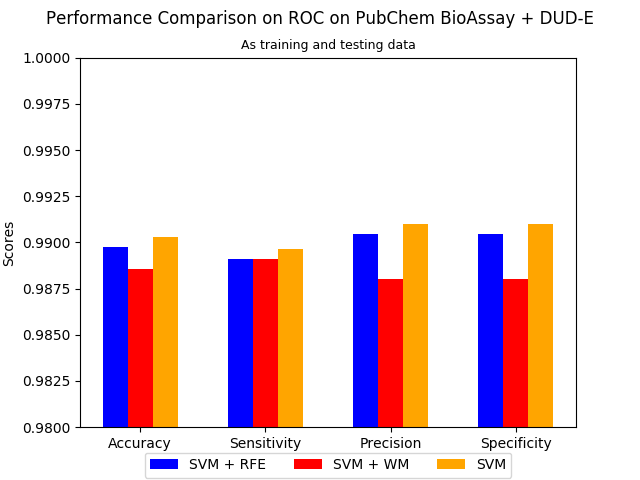
\includegraphics[scale=0.5]{../images/03-evaluate-1_scores_chart.png}
	\caption{Classification performance comparison on PubChem BioAssay + DUD-E dataset}
	\label{fig_performance_comparison_pubchem}
\end{figure}

\begin{figure}
	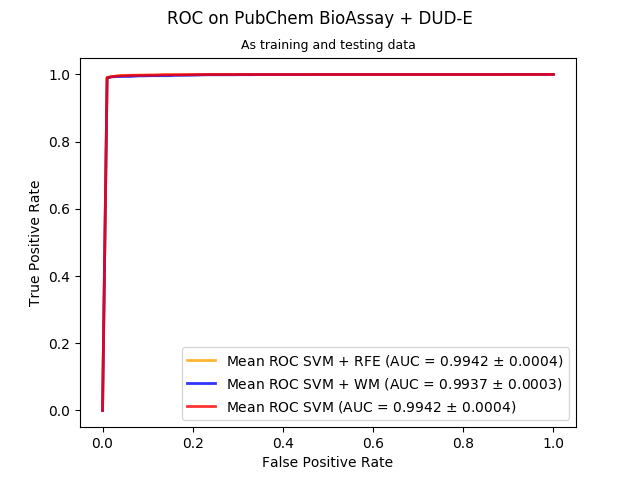
\includegraphics[scale=0.5]{../images/03-evaluate-1_roc_chart.png}
	\caption{AUC ROC comparison on PubChem BioAssay + DUD-E dataset}
	\label{fig_roc_comparison_pubchem}
\end{figure}


\begin{figure}
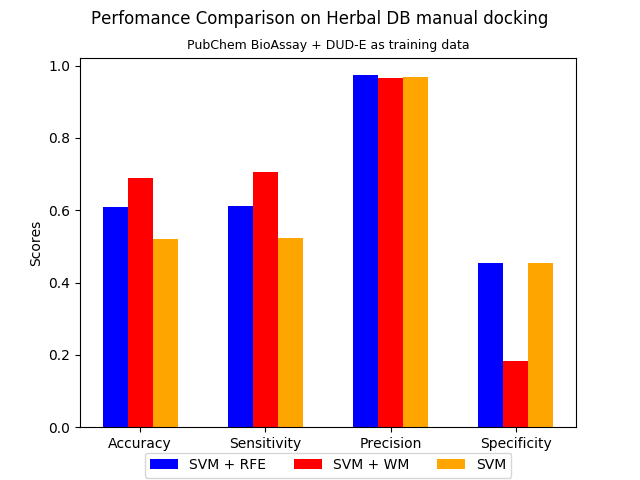
\includegraphics[scale=0.5]{../images/03-evaluate-3_scores_chart.png}
\caption{Classification performance comparison on Herbal DB dataset}
\label{fig_performance_comparison_herbaldb}
\end{figure}

\begin{figure}
	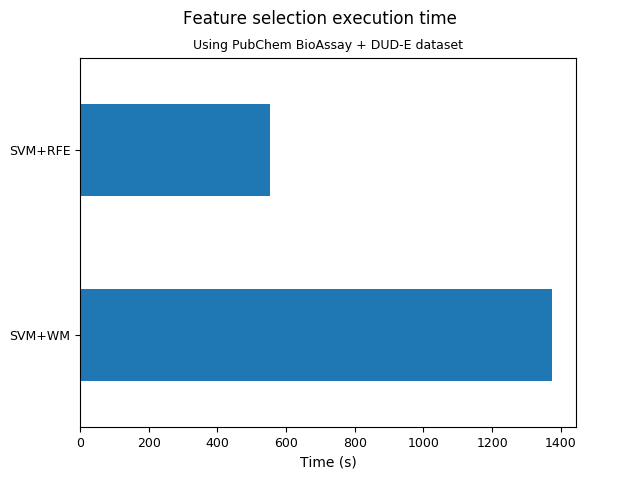
\includegraphics[scale=0.5]{../images/feature_selection_time_comparison.png}
	\caption{Feature selection time comparison}
	\label{fig_feature_selection_time_comparison}
\end{figure}

\begin{figure}
	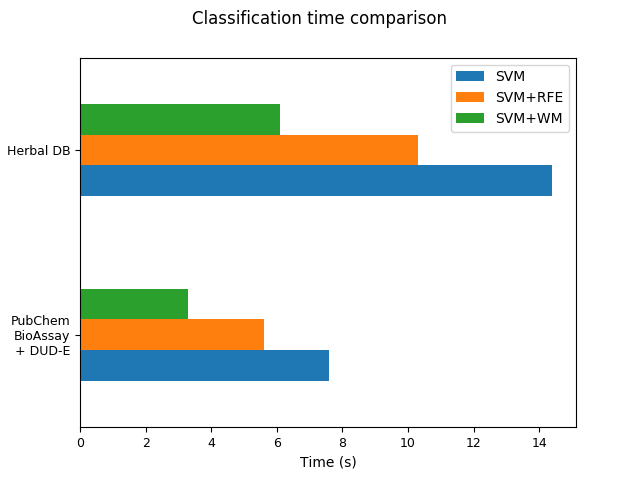
\includegraphics[scale=0.5]{../images/classification_time_comparison.png}
	\caption{Classification time comparison}
	\label{fig_classification_time_comparison}
\end{figure}

\section{Analysis}

TODO

Model mana yang paling akurat memprediksi hasil docking senyawa dengan HIV-1

\section{Conclusion}

TODO

% conference papers do not normally have an appendix

% use section* for acknowledgment
%\ifCLASSOPTIONcompsoc
  % The Computer Society usually uses the plural form
%  \section*{Acknowledgments}
%\else
  % regular IEEE prefers the singular form
%  \section*{Acknowledgment}
%\fi

\bibliographystyle{IEEEtran}
\bibliography{../references}

% that's all folks
\end{document}
